%Este arquivo deve ser alterado pelos integrantes da respectiva equipe com o conteudo indicado abaixo.
%Equipe: Sergio Luis, Inácio

%Livro: Seção 5.3.1, p.129

%Inserir no arquivo \textbf{modelo\_periodico.tex} a descrição do modelo TCP
%periódico.
Este é o modelo mais simples para o TCP, que considera o padrão periódico na
dinâmica da janela de congestionamento e a perda de pacotes. Não é levada em
conta nenhuma versão específica do TCP, mas apenas a dinâmica comum a todas
estas versões, ou seja, a maneira como a janela decresce multiplicativamente a
cada perda periódica de pacote. Como estamos considerando o estado estacionário
(\textit{steady-state}), um tamanho de janela máximo $W$ é sempre atingido no
momento em que um pacote é perdido, e isso resulta na redução da janela pela
metade, ou seja, $\frac{W}{2}$. Além disso, a operação do sistema no estado
estacionário implica que as perdas de pacotes ocorrem com probabilidade
constante $p$, tal que, em média, $\frac{1}{p}$ pacotes são transmitidos na rede
entre cada perda de pacote (Equação \ref{media}). Lembrando que na perda de
pacote, a janela é reduzida. Também é importante lembrar que, como estamos considerando o estado
estacionário, significa que atingimos um padrão regular, que persiste por todo o
tempo, ou seja, não é levado em consideração a partida lenta
(\textit{slow-start}), por exemplo, mas apenas o estado final, estável, com o
tamanho máximo da janela já atingido.

\begin{align}
\label{media}
numero\ medio\ de\ pacotes\ transmitidos &= \sum_{k=1}^{\infty}
\left[(1-p)^{k-1}p\right] \cdot k \nonumber\\
&= \frac{p}{(1-p)} \sum_{k=1}^{\infty} (1-p)^{k} \cdot k\nonumber\\
&= \frac{p}{1-p} \cdot \frac{1-p}{\left(1-(1-p)\right)^{2}}\nonumber\\
&= \frac{p}{p^{2}} = \frac{1}{p}
\end{align}

Se plotarmos a variação da janela em função do tempo, no estado
estacionário, observaremos a forma ``dente de serra'' (Figura \ref{serra}) do
TCP. Apesar do modelo periódico ser menos realista, ele permite que derivemos uma propriedade
fundamental com relação ao desemprenho do TCP, que é conhecida como a
\textit{lei da raiz quadrada inversa de p}.

\begin{figure}
\label{serra}
\centering
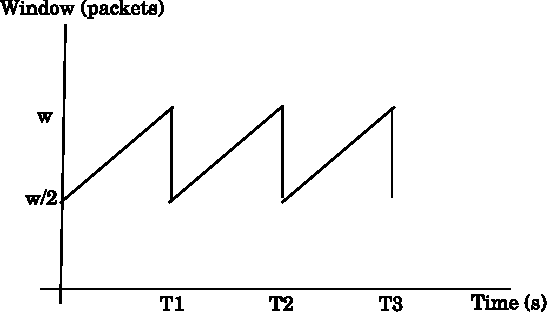
\includegraphics{figs/periodic_model.pdf}
\caption{Modelo periódico do TCP}
\end{figure}

Devido à forma periódica da dinâmica da janela no estado estacionário, o
desempenho do TCP nestas condições pode ser derivado determinando o número de
pacotes transmitidos em um perído, e o comprimento do período. Como temos uma
probabilidade constante ($p$) para a perda de pacotes, o número de pacotes é
dado por $\frac{1}{p}$, como dito anteriormente, porque nós temos que transmitir
esta quantidade de pacotes antes que um pacotes seja perdido. Uma maneira
alternativa de se encontrar o número total de pacotes transmitidos em um período
é encontrar a área sob o rastro do tamanho da janela, o que é bem simples,
devido à forma trapezoidal (um trapézio de bases $W$  e $\frac{W}{2}$  e
altura $T$) do período. Em um trapézio de bases $b_1$ e $b_2$ e altura $h$,
temos que sua área é dada por:

$$\frac{(b_1 + b_2)}{2}\cdot h$$

Logo, temos que o número de pacotes transmitidos em um período é o seguinte:
\begin{equation}
\label{npkt}
Numero\ de\ pacotes = \frac{1}{2}\frac{T}{RTT}\left(\frac{W}{2} + W\right)
\end{equation}

Onde $T$ é o período entre as perdas detectadas. O tempo deve ser escalado pelo
$RTT$ (\textit{round-trip time}), já que a fonte TCP não envia pacotes
continuamente, e o tempo deve avançar pelo período de um RTT antes que um
conjunto totalmente novo de pacotes, contido pelo tamanho da janela, contribua
com o número total de pacotes transmitido. Como sabemos que o TCP aumenta sua
janela na taxa de um pacote por RTT durante sua fase de crescimento linear, o
tempo que leva para aumentar a janela de $\frac{W}{2}$ para $W$ é $T =
RTT \cdot \frac{W}{2}$. 

Substituindo o valor de $T$ na Fórmula (\ref{npkt}), temos que o número de
pacotes enviados em um período é o seguinte:
\begin{align}
\label{npkt2}
numero\ de\ pacotes &= \frac{1}{2}\frac{RTT \cdot
\frac{W}{2}}{RTT}\left(\frac{W}{2} + W\right)\nonumber\\
				&= \frac{W}{4} \cdot \left(\frac{W}{2} + W\right)
\end{align} 

 Logo, igualando o número total de pacotes transmitidos
durante esse período (Equações \ref{npkt2} e \ref{media}), temos:
\begin{align}
\frac{W}{4} \cdot \left(\frac{W}{2} + W\right) &= \frac{1}{p}\nonumber\\
\Rightarrow W &= \sqrt{\frac{8}{3p}}
\end{align}

Nós podemos agora achar a taxa média de envio $\bar{X}(p)$ da fonte TCP, que é o
número de pacotes transmitidos a cada período:
\begin{align}
\bar{X}(p) &= \frac{pacotes\ enviados\ em\ media}{tempo}\nonumber\\ 
	&= \frac{\frac{1}{p}}{RTT \cdot \frac{W}{2}}\nonumber\\
			&= \frac{1}{RTT} \sqrt{\frac{3}{2p}}
\end{align}

Este resultado é conhecido como a \textit{lei da raiz quadrada inversa de p}, e,
em particular, mostra que a taxa de transmissão de uma fonte TCP é inversamente
relacionada ao RTT e a raiz quadrada da probabilidade média de perda de um
pacote.
